\documentclass[conference]{IEEEtran}
\IEEEoverridecommandlockouts
% The preceding line is only needed to identify funding in the first footnote. If that is unneeded, please comment it out.
\usepackage{cite}
\usepackage{amsmath,amssymb,amsfonts}
\usepackage{algorithmic}
\usepackage{graphicx}
\usepackage{textcomp}
\usepackage{xcolor}
\usepackage{url}
\usepackage{float}
\usepackage{comment}
\def\BibTeX{{\rm B\kern-.05em{\sc i\kern-.025em b}\kern-.08em
    T\kern-.1667em\lower.7ex\hbox{E}\kern-.125emX}}
\begin{document}

\title{Simulated Annealing}

\author{\IEEEauthorblockN{Heansuh Lee}
\IEEEauthorblockA{\textit{Electronic Engineering} \\
\textit{Hochschule Hamm-Lippstadt}\\
Lippstadt, Germany \\
heansuh.lee@stud.hshl.de}

}

\maketitle

\begin{abstract}
Simulated annealing - what is it about?

Since its introduction as a generic heuristic for discrete optimization in 1983, simulated annealing (SA) has become a popular tool for tackling both discrete and continuous problems across a broad range of application areas.  The use of simulated annealing in the solution of practical problems will be covered. A detailed statement of the algorithm is given, together with an explanation of its inspiration from the field of statistical thermodynamics. This is followed by a brief overview of the theory with emphasis on those results that are important to the decisions that need to be made for a practical implementation. It then goes on to look at some of the ways in which the basic algorithm has been modified in order to improve its performance in the solution of a variety of problems.
\end{abstract}

\begin{IEEEkeywords}
HLS, algorithm, AI, annealing, Python
\end{IEEEkeywords}

\section{Introduction}
This document describes simulated annealing (abbreviated as SA) in terms of: (1) definition, and (2) history of SA.

\subsection{Definition}
Simulated annealing is one of the High-Level Synthesis (HLS) algorithms. SA is a probabilistic technique for approximating the global optimum of a given function. Specifically, it is a metaheuristic to approximate global optimization in a large search space for an optimization problem \cite{b1}.

\subsection{History}
In the early 1980s, three IBM researchers, Kirkpatrick et al. \cite{b2}, introduced the concepts of annealing in combinatorial optimization. These concepts are based on a strong analogy with the physical annealing of materials. This process involves bringing a solid to a low energy state after raising its temperature. It can be summarised by the following two steps:
\begin{itemize}
    \item Bring the solid to a very high temperature until “melting” of the structure;
    \item Cool the solid according to a very particular temperature decreasing scheme in order to reach a solid state of minimum energy.
\end{itemize}

In the liquid phase, the particles are distributed randomly. It is shown that the minimum-energy state is reached provided that the initial temperature is sufficiently high and the cooling time is sufficiently long. If this is not the case, the solid will be
found in ametastable state with non-minimal energy; this is referred to as hardening, which consists in the sudden cooling of a solid.

\begin{figure}[H]
\centerline{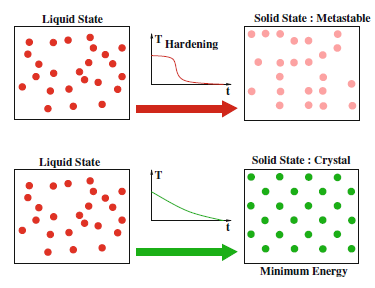
\includegraphics[width=0.45\textwidth,height=0.45\textheight,keepaspectratio]{fig1.png}}
\caption{When the temperature is high, the material is in a liquid state (left). For a hardening process, the material reaches a solid state with non-minimal energy (metastable state; top right). In
this case, the structure of the atoms has no symmetry. During a slow annealing process, the material reaches also a solid state but for which atoms are organized with symmetry (crystal; bottom right)}
\end{figure}


\section{Model-based Design}

There are model-based designs to describe simulated annealing.

\subsection{Analogy to a Toy}

\begin{figure}[H]
\centerline{
\includegraphics[width=0.2\textwidth,height=0.2\textheight,keepaspectratio]{fig2.jpg}}
\caption{An image of a water ring toss game toy \cite{b3}.}
\end{figure}

Analogy to a toy \cite{b4}. 

\subsection{Solving Sudoku}

Solving sudoku \cite{b5}.

\section{Simulated Annealing Algorithm}

Before describing the simulated annealing algorithm for optimization, there will be an introduction of the principles of local search optimization algorithms, of which simulated annealing is an extension.

\subsection{Local Search (or Monte Carlo) Algorithms}

These algorithms optimize the cost function by exploring the neighborhood of the current point in the solution space.

In the next definitions, we consider ($S$, $f$) an instantiation of a combinatorial optimization problem ($S$: set of feasible solutions, $f$: objective function to be minimized).

\textbf{Definition 1} Let $N$ be an application that defines for each solution $i$ ∈ $S$ a subset $S_{i}$ ⊂ $S$ of solutions “close” (to be defined by the user according to the problem of interest) to the solution $i$. The subset $S_{i}$ is called the neighborhood of solution $i$.

In the next definitions, we consider that $N$ is a neighborhood structure associated with ($S$, $f$).

\textbf{Definition 2} A generating mechanism is a mean for selecting a solution $j$ in any neighborhood $S_{i}$ of a given solution $i$.

A local search algorithm is an iterative algorithm that begins its search from a feasible point, randomly drawn in the state space. A generation mechanism is then successively applied in order to find a better solution (in terms of the objective function value), by exploring the neighborhood of the current solution. If such a solution is found, it becomes the current solution. The algorithm ends when no improvement can be found, and the current solution is considered as the approximate solution of the optimization problem. One can summarise the algorithm by the following pseudo-code for a minimization problem:

\textbf{Local Search}

\begin{enumerate}
\item Draw an initial solution $i$;
\item Generate a solution $j$ from the neighborhood $S_{i}$ of the current solution $i$;
\item If $f$($j$) < $f$($i$) then $j$ becomes the current solution;
\item If $f$($j$) ≥ $f$($i$) for all $j$ ∈ $S_{i^{*}}$ then END;
\item Go to step 2;
\end{enumerate}

\textbf{Definition 3} A solution $i^{*}$ ∈ $S$ is called a local optimum with respect to $N$ for ($S$, $f$) if $f$($i^{*}$) ≤ $f$ ($j$) for all $j$ ∈ $S_{i}$.

\textbf{Definition 4} The neighborhood structure $N$ is said to be exact if, for every local optimum with respect to $N$, $i$ ∈ $S$, $i^{*}$ is also a global optimum of ($S$,$f$).

Thus, by definition, local search algorithms converge to local optima unless one has an exact neighborhood structure. This notion of exact neighborhood is theoretical because it generally leads, in practice, to resort to a complete enumeration of the
search space.

Intuitively, if the current solution “falls” in a subdomain over which the objective function is convex, the algorithm remains trapped in this subdomain, unless the neighborhood structure associated with the generation mechanism can reach points
outside this subdomain.

In order to avoid being trapped in local minima, it is then necessary to define a process likely to accept current state transitions that momentarily reduce the performance (in terms of objective) of the current solution: this is the main principle of
simulated annealing.

\subsection{Metropolis Algorithm}
Before describing this algorithm, it is necessary to introduce the Metropolis algorithm \cite{b6}, which is a basic component of SA.

In 1953, three American researchers developed this algorithm to simulate the physical annealing process. Their aim was to reproduce faithfully the evolution of the physical structure of a material undergoing annealing.

This algorithm is based on Monte Carlo techniques which consist in generating a sequence of states of the solid in the following way.

Starting from an initial state $i$ of energy $E_{i}$, a new state $j$ of energy $E_{j}$ is generated by modifying the position of one particle.

If the energy difference, $E_{i}$ − $E_{j}$ , is positive (the new state features lower energy), the state $j$ becomes the new current state. If the energy difference is less than or equal to zero, then the probability that the state j becomes the current state is given by:

$P_{r}$ (Current state = $j$) = $e^((E_i-E_j)/(k_bT))$
...
page 5

\subsection{Simulated Annealing (SA) Algorithm}

In the SA algorithm, the Metropolis algorithm is applied to generate a sequence of solutions in the state space $S$. To do this, an analogy is made between a multi-particle system and our optimization problem by using the following equivalences:

\begin{itemize}
    \item The state-space points (solutions) represent the possible states of the solid;
    \item The function to be minimized represents the energy of the solid.
\end{itemize}

A control parameter $c$, acting as a temperature, is then introduced. This parameter is expressed with the same units as the objective that is optimized.

It is also assumed that the user provides for each point of the state space, a neighborhood and a mechanism for generating a solution in this neighborhood. We then define the acceptance principle:

\textbf{Definition 5} \textit{Let ($S$,$f$) be an instantiation of a combinatorial minimization problem, and $i$, $j$ two points of the state space. The acceptance criterion for accepting solution $j$ from the current solution $i$ is given by the following probability:}

eqn

By analogy, the principle of generation of a neighbor corresponds to the perturbation mechanism of the Metropolis algorithm, and the principle of acceptance represents the Metropolis criterion.

...
pg 6

\subsection{Travelling Salesman problem (TSP}
The traveling salesman problem (TSP) asks the following question: “Given a list of $n$ cities, among which an origin city, and the distances between each pair of cities, what is the shortest possible route that visits each city exactly once and returns to
the origin city?” This is again an important NP-hard combinatorial optimization problem, particularly in the fields of operations research and theoretical computer science. The problem was first formulated in 1930 and is one of the most intensively studied problems in discrete optimization \cite{b7}.

\begin{figure}[H]
\centerline{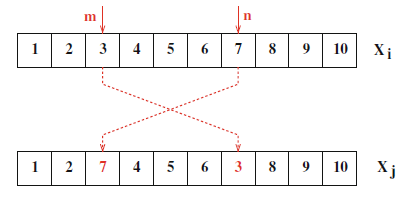
\includegraphics[width=0.45\textwidth,height=0.45\textheight,keepaspectratio]{fig3.png}}
\caption{A first neighborhood operator: randomly swapping two positions [p.26,1].}
\end{figure}

\begin{figure}[H]
\centerline{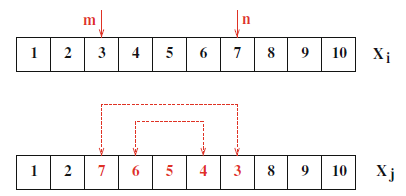
\includegraphics[width=0.45\textwidth,height=0.45\textheight,keepaspectratio]{fig4.png}}
\caption{A second neighborhood operator: swapping all positions between two randomly chosen positions ($m$,$n$) [p.26,1].}
\end{figure}

\begin{figure}[H]
\centerline{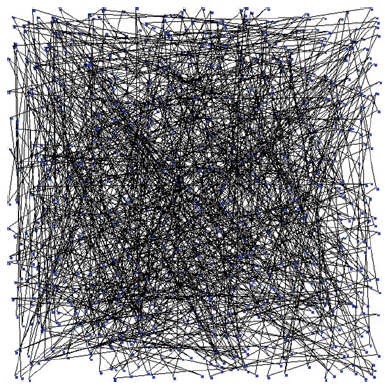
\includegraphics[width=0.45\textwidth,height=0.45\textheight,keepaspectratio]{fig5.png}}
\caption{Initial tour of the TSP with n = 1000 cities [p.26,1].}
\end{figure}

\begin{figure}[H]
\centerline{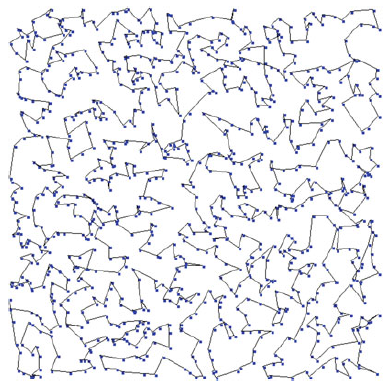
\includegraphics[width=0.45\textwidth,height=0.45\textheight,keepaspectratio]{fig6.png}}
\caption{Final tour of the TSP with n = 1000 cities [p.27,1]}
\end{figure}



\section{Uses}

- real-life examples \cite{b8}.

\subsection{Artificial Intelligence}
in the field of AI \cite{b9}

\subsection{Search Function in Python}
- used in python as well for search functions \cite{b10}.

\section{Advantages}
- talk about advantages

\section{Constraints}
- computational issues occur from using it

\section{Evaluation}
- evaluate pros and cons, and see if it's used currently, or compare to other technology

\section{Conclusion}
- summary of the whole paper

\begin{thebibliography}{00}
\bibitem{b1} M. Gendreau and J.-Y. Potvin, Handbook of metaheuristics. Cham, Switzerland: Springer, 2019. 

\begin{comment}
\url{https://link.springer.com/referenceworkentry/10.1007%2F978-3-540-92910-9_49}.
\end{comment}

\bibitem{b2} S. Kirkpatrick, C. Gelatt, and M. Vecchi, Optimization by simulated annealing. IBM Research Report RC 9355, Acts of PTRC Summer Annual Meeting, 1982.
\bibitem{b3} 2 Pieces Water Handheld Game Mini Water Ring Game Water Ring Toss and Basketball Aqua Arcade Toy for Party Favor Fun Game for Most Ages, Without Water. Available: \url{https://images-na.ssl-images-amazon.com/images/I/71tEp%2BBaL7L.jpg}, Accessed on: May 19, 2021.
\begin{comment}
\url{https://www.youtube.com/watch?v=FyyVbuLZav8}.
\end{comment}
\bibitem{b4} \url{https://link.springer.com/chapter/10.1007/978-3-319-91086-4_1}.
\bibitem{b5} \url{https://mathworld.wolfram.com/SimulatedAnnealing.html#:~:text=A%20typical%20example%20is%20the,heated%20and%20then%20slowly%20cooled).}.
\bibitem{b6} N. Metropolis, A. W. Rosenbluth, M. N. Rosenbluth, A. H. Teller, and E. Teller, “Equation of state calculations by fast computing machines,” 1953. 
\begin{comment}
\url{\url{https://link.springer.com/chapter/10.1007/978-3-319-91086-4_1#:~:text=Simulated%20Annealing%20(SA)%20is%20one,used%20in%20real%2Dlife%20applications.}.}.
\end{comment}
\bibitem{b7} \url{https://www.youtube.com/watch?v=S9vs05eAGN0}.
\bibitem{b8} \url{https://www.youtube.com/watch?v=C86j1AoMRr0}.

\end{thebibliography}

\end{document}
